% Compile with: tectonic ta_checkin.tex
% Or: latexmk -pdf ta_checkin.tex
% Speaker notes are included in the source but hidden in the presentation PDF.
\documentclass[aspectratio=169,11pt]{beamer}
\usetheme{Boadilla}
\usepackage[T1]{fontenc}
\usepackage{lmodern}
\usepackage{booktabs,tabularx,array}
\usepackage{graphicx}
\usepackage{pgfplots}
\pgfplotsset{compat=1.18}
\definecolor{forest}{HTML}{24382D}
\definecolor{rust}{HTML}{AF573D}
\definecolor{muted}{HTML}{686D60}
\setbeamercolor{normal text}{fg=forest,bg=white}
\setbeamercolor{structure}{fg=forest}
\setbeamercolor{alerted text}{fg=rust}
\setbeamercolor{frametitle}{fg=forest,bg=white}
\setbeamercolor{title}{fg=forest}
\setbeamerfont{frametitle}{size=\Large,series=\bfseries}
\setbeamertemplate{navigation symbols}{}
\setbeamertemplate{headline}{}
\setbeamertemplate{footline}{\hspace{7mm}\color{muted}\scriptsize CIS 5810\hfill\insertframenumber/\inserttotalframenumber\hspace{7mm}\vspace{3mm}}
\setbeamersize{text margin left=7mm,text margin right=7mm}
\setbeameroption{hide notes}
\newcommand{\source}[1]{\par\vfill{\fontsize{7}{8}\selectfont\color{muted}#1\par}}
\newcommand{\repo}[2]{\href{https://github.com/aking526/ai-camera-roll/blob/84bd89bb9e947a0866aca6654ffc04a3a5d9119f/#1}{#2}}
\hypersetup{pdftitle={CIS 5810: Making character consistency measurable},pdfauthor={Ethan Wei, Alistair King, Tanay Tandon},colorlinks=true,urlcolor=forest}

\begin{document}

\begin{frame}
\begin{columns}[c,onlytextwidth]
\begin{column}{.53\textwidth}
{\small CIS 5810 TA check-in \textbar\ Group 30\par}
\vspace{6mm}
{\LARGE\bfseries Making character\\consistency measurable\par}
\vspace{5mm}
Iteration 01: portrait retention tested\par
\vspace{1mm}
Scoring implemented.\\Mixed result; validate next.\par
\vspace{7mm}
{\small Ethan Wei, Alistair King\\Tanay Tandon\par}
\vspace{2mm}
{\small November 2026}
\end{column}
\begin{column}{.44\textwidth}
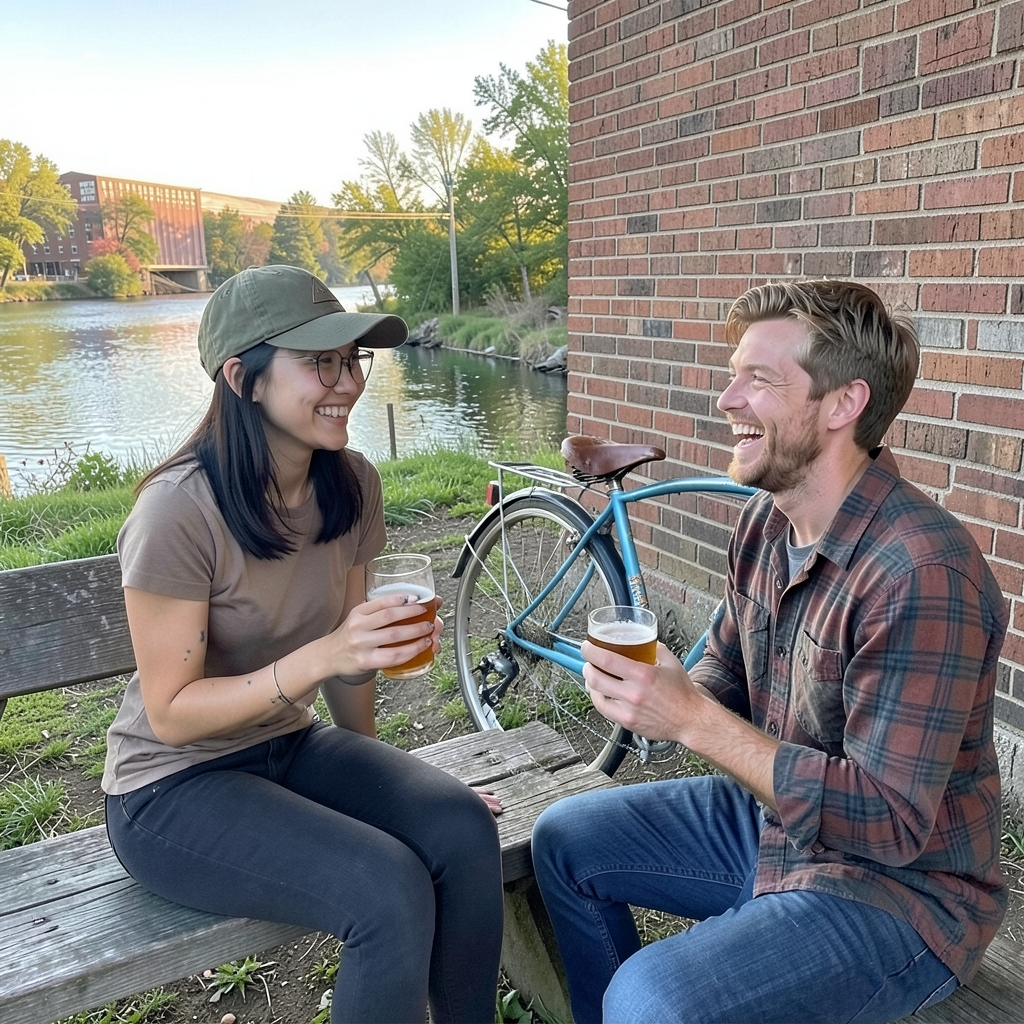
\includegraphics[width=\linewidth]{assets/maya_may.png}
\end{column}
\end{columns}
\note{We already had a working reference-conditioned, multi-pass camera-roll pipeline at the proposal. This update makes its output measurable and inspectable. We have not yet demonstrated a quality improvement. The cover is an existing synthetic May scene, not a new generation. Sources: project proposal pages 1--3 and the saved Maya pilot.}
\end{frame}

\begin{frame}{What existed and what we added}
\renewcommand{\arraystretch}{1.4}
\small
\begin{tabularx}{\textwidth}{@{}>{\raggedright\arraybackslash}X >{\raggedright\arraybackslash}X@{}}
\toprule
\textbf{Existing before this work} & \textbf{Added during this work}\\
\midrule
Story, scene prompts, canonical portraits and reference-conditioned editing & SCRFD and ArcFace scoring of all nine saved passes, with crops and candidate matches\\
Saved passes, prompts and a technical camera-roll viewer & Story-first website with face and object score comparisons\\
Proposed identity-retention experiment & Controlled portrait-reference comparison with preserved images, prompts and scoring evidence\\
\bottomrule
\end{tabularx}\par
\vspace{5mm}
\normalsize\textbf{Existing Maya pilot:} five scenes, eight references, nine scene passes.
\source{Sources: proposal pp. 1--3; \repo{evaluation/README.md}{evaluation documentation}; \repo{demo_site/RATING_GUIDE.txt}{rating guide}.}
\note{The proposal described five text-only baseline images, followed by a reference-conditioned iteration with a prompt compiler, canonical references and editing passes. The displayed Maya pilot is that reference-conditioned version. We did not recover the original text-only images, so we do not claim a new quantified comparison with them. ArcFace was already proposed; this work implements that plan. CLIP and SAM remain proposed methods. The original technical viewer is established by repository evidence, not the proposal text. No independent rating result or new image-quality improvement is claimed.}
\end{frame}

\begin{frame}{How we measure face consistency}
\raggedright
\textbf{1. SCRFD finds faces.} It locates faces and landmarks such as the eyes and nose. We use these landmarks to crop and align each face consistently.\par
\vspace{3mm}
\textbf{2. ArcFace describes identity.} A pretrained recognition network converts each face into a compact set of numbers. Its training encourages images of the same person to have similar representations.\par
\vspace{3mm}
\textbf{3. Compare with the portrait.} We compare those numbers with the character's reference using cosine similarity. The score ranges from $-1$ to $1$. Higher means a closer model match.\par
\vspace{2mm}
\small\textbf{Why these tools?} Efficient face detection and identity-focused comparison, with pretrained models that run locally and score every pass consistently.
\vspace{2mm}
\par\alert{Human review checks whether score changes reflect identity changes.}
\source{Sources: \href{https://arxiv.org/abs/2105.04714}{SCRFD paper}; \href{https://arxiv.org/abs/1801.07698}{ArcFace paper}; \repo{evaluation/score_faces.py}{local evaluator}.}
\note{SCRFD is the face detector. Its efficient design makes local evaluation practical, and its landmarks support repeatable alignment. ArcFace is the recognition method: its pretrained network learns facial features useful for distinguishing identities. We chose face-specific comparison because character identity is the target, rather than overall scene similarity. Both are available together through InsightFace and require no generation API calls to score the saved images. The local setup uses SCRFD-10GF and ArcFace ResNet50 from buffalo\_l, with 112 by 112 aligned crops. Cosine similarity compares the learned numerical descriptions. The evaluator builds all reference-to-candidate comparisons and chooses a one-to-one assignment. Assigned candidates can still be weak matches. Scores are not identity probabilities, and we have no calibrated identity cutoff. Pose, visibility and alignment can affect them. Neither model was specifically trained or validated here for synthetic character identity.}
\end{frame}

\begin{frame}{The two models at a glance}
\begin{columns}[t,onlytextwidth]
\begin{column}{.47\textwidth}
\textbf{SCRFD} \quad {\small Face detection}\par
\vspace{4mm}
Finds faces in an image and estimates facial landmarks, including the eyes and nose.\par
\vspace{4mm}
\textbf{In our pipeline:} locate, crop and align each face before scoring.
\end{column}
\begin{column}{.47\textwidth}
\textbf{ArcFace} \quad {\small Face recognition}\par
\vspace{4mm}
Encodes an aligned face as a numerical representation designed to distinguish identities.\par
\vspace{4mm}
\textbf{In our pipeline:} compare the candidate and reference representations using cosine similarity.
\end{column}
\end{columns}
\source{Sources: \href{https://arxiv.org/abs/2105.04714}{SCRFD paper}; \href{https://arxiv.org/abs/1801.07698}{ArcFace paper}.}
\note{SCRFD provides bounding boxes and landmarks; the landmarks allow consistent face alignment. ArcFace maps aligned faces into an embedding space where cosine similarity can be used to compare them. The resulting score is a model similarity, not a probability of identity.}
\end{frame}

\begin{frame}{Historical pilot: Maya's score fell in four edited scenes}
\small First pass versus final pass. Higher similarity means a closer model match.
\vspace{2mm}
\begin{center}
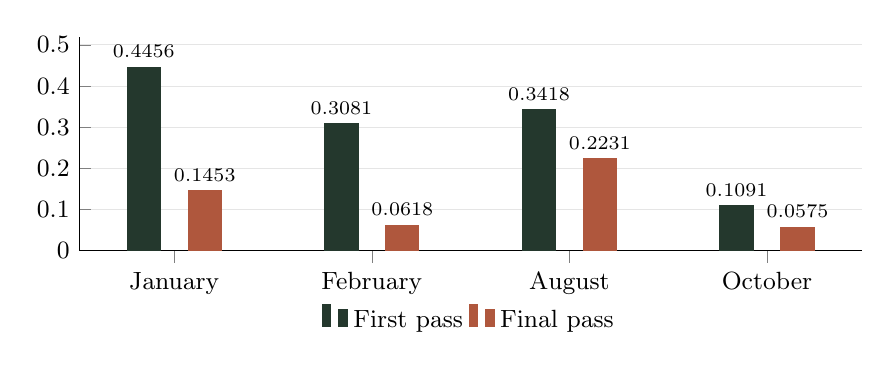
\begin{tikzpicture}
\begin{axis}[
 width=.95\textwidth,height=43mm,
ybar=10pt,bar width=12pt,ymin=0,ymax=.52,
 ytick={0,.1,.2,.3,.4,.5},
 symbolic x coords={January,February,August,October},xtick=data,
 enlarge x limits=.16,
 axis lines*=left,ymajorgrids=true,grid style={gray!20},
 tick label style={font=\small},
 nodes near coords,point meta=y,
 every node near coord/.append style={font=\scriptsize,/pgf/number format/fixed,/pgf/number format/precision=4,/pgf/number format/zerofill},
 legend style={at={(.5,-.22)},anchor=north,legend columns=2,draw=none,font=\small},
 ]
\addplot[fill=forest,draw=forest] coordinates {(January,.4455871328864703) (February,.30807495358305204) (August,.34181872034847716) (October,.10911143299338712)};
\addplot[fill=rust,draw=rust] coordinates {(January,.14525147558402593) (February,.06178808040049918) (August,.22305779596064895) (October,.05748159883324351)};
\legend{First pass,Final pass}
\end{axis}
\end{tikzpicture}
\end{center}
\vspace{3mm}
\small May: 0.3098, single pass. No before/after comparison.\par
\vspace{1mm}
\alert{This historical signal motivated the controlled portrait-retention test.}
\source{Source: \repo{evaluation/results/scores.json}{saved ArcFace results}. Scores compare assigned candidates with Maya's canonical portrait.}
\note{January has the largest observed decrease: .4456 to .1453, a change of -.3003. All four edited scenes show lower assigned Maya similarity after the edit. May is single-pass and must not be treated as zero change. These are model observations, not independent human judgments or evidence of causality. The chart shows the observed positive range, while cosine similarity can range from -1 to 1. Pose, visibility, alignment and assignment can affect scores.}
\end{frame}

\begin{frame}{January: a controlled comparison of the portrait edit}
\centering
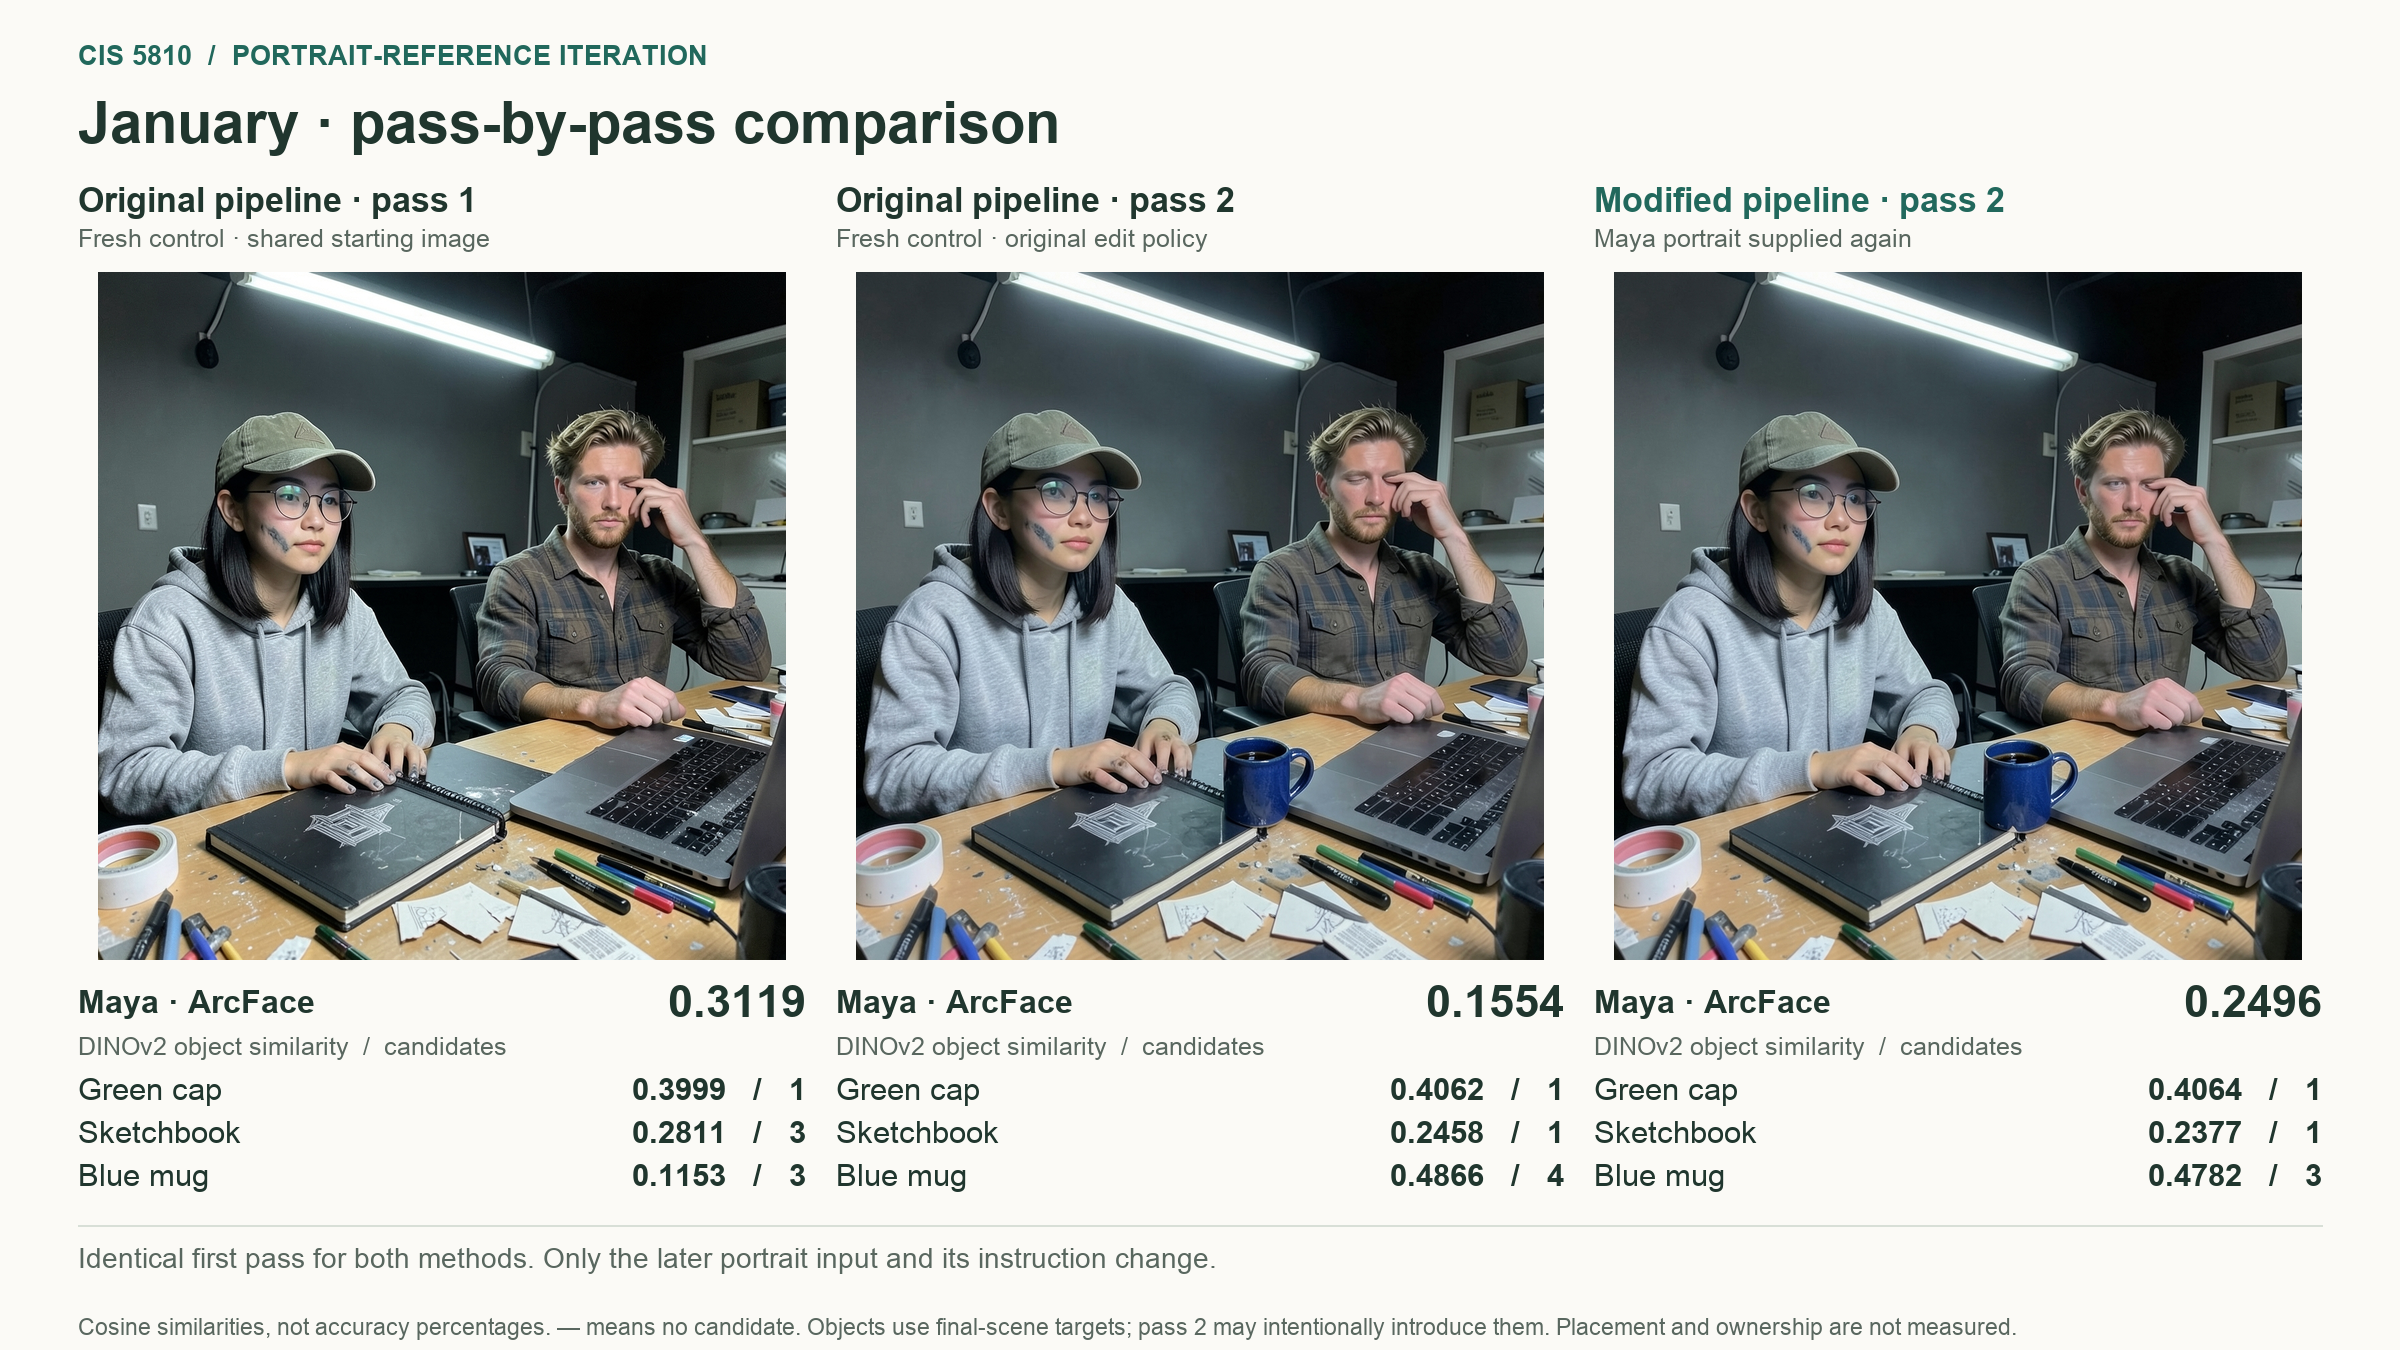
\includegraphics[width=.98\textwidth,height=.72\textheight,keepaspectratio]{../experiments/iteration_01_portrait_retention_2026-11-04/figures/01_01_comparison.png}
\source{Same first-pass image in both conditions; only the portrait input and its instruction changed. Source: \repo{experiments/iteration_01_portrait_retention_2026-11-04/README.md}{Iteration 01 evidence package}.}
\note{This is a fresh controlled replay, not a comparison against the older historical pilot. The original second pass reduces Maya's ArcFace cosine from 0.3119 to 0.1554. Supplying Maya's portrait again produces 0.2496, a partial recovery. Object resemblance values are model scores and do not verify placement or ownership.}
\end{frame}

\begin{frame}{Portrait retention partly recovered face similarity}
\small
\begin{center}
\renewcommand{\arraystretch}{1.35}
\begin{tabular}{lrrr}
\toprule
\textbf{Scene} & \textbf{Shared pass 1} & \textbf{Original pass 2} & \textbf{Portrait pass 2}\\
\midrule
January & .3119 & .1554 & .2496\\
February & .1973 & .0910 & .1743\\
August & .1002 & .0726 & .1106\\
October & .1277 & .1284 & .2039*\\
\bottomrule
\end{tabular}
\end{center}
\vspace{3mm}
\textbf{Same-candidate scenes:} mean .1063 $\rightarrow$ .1782 after the change; still below the shared first-pass mean (.2031).
\vspace{3mm}
\alert{October is a matcher failure: it selected another person. The intended person's score fell .1284 $\rightarrow$ .0696.}
\source{ArcFace cosine similarities, not accuracy percentages. Three-scene subset is post-hoc. One five-scene run; no repeated trials or confidence intervals. Source: \repo{experiments/iteration_01_portrait_retention_2026-11-04/ANALYSIS.md}{analysis and limitations}.}
\note{The three-scene mean uses January, February and August, where Maya keeps the same candidate index. This is a post-hoc subset, not a preregistered success rate. October's Hungarian assignment switched Maya from the left-hand cook to the center person in scrubs, so the assigned .2039 is not a valid improvement. Position-based diagnostic for the intended cook is .0696, down from .1284. Keep this caveat next to the headline result.}
\end{frame}

\begin{frame}{Object resemblance stayed essentially unchanged}
\begin{columns}[t,onlytextwidth]
\begin{column}{.47\textwidth}
\textbf{Matched edited-scene objects}\par
\vspace{4mm}
Same 10 appearances with candidates in both conditions; shared May excluded.\par
\vspace{5mm}
\Large\textbf{.3064 $\rightarrow$ .3045}\par
Mean DINOv2 cosine similarity\par
\vspace{3mm}
Change: $-0.0020$.
\end{column}
\begin{column}{.47\textwidth}
\textbf{What the score cannot tell us}\par
\vspace{4mm}
It measures resemblance to one reference view. It does not verify object placement, owner, count or state.\par
\vspace{4mm}
In February, the mug moved from the requested radiator to Maya's hand; its score fell .5153 $\rightarrow$ .3317.
\end{column}
\end{columns}
\source{Localization: Grounding DINO. Similarity: DINOv2 on selected crops. Source: \repo{experiments/iteration_01_portrait_retention_2026-11-04/ANALYSIS.md}{object results and caveats}.}
\note{Object candidate coverage was 12/13 for both final sets, but this does not prove presence: the blank-image sanity check produced false positives. The fair comparison matches ten appearances with candidates in both conditions and excludes shared May. Average resemblance is essentially flat. Some individual objects improved while others declined. We should not claim an object-quality gain.}
\end{frame}

\begin{frame}{Human judgments help interpret the scores}
\raggedright
\textbf{Automated comparisons are reproducible.} The package preserves images, prompts, manifests, model outputs and matched scores.\par
\vspace{5mm}
\textbf{Human review is still needed.} Check identity, object count, placement and state, plus setting and action.\par
\vspace{5mm}
\textbf{Uncertainty stays visible.} Allow unclear judgments. Retain raw votes, disagreements and prior-exposure disclosures.\par
\vspace{3mm}
\alert{No independent human ratings or repeated generation trials are included yet.}\par
\small Keep portrait retention experimental; the evidence shows partial recovery and meaningful failure cases.
\source{Source: \repo{experiments/iteration_01_portrait_retention_2026-11-04/ANALYSIS.md}{study limits}; \repo{demo_site/RATING_GUIDE.txt}{rating guide}.}
\note{The evidence package includes assistant visual observations, not independent human ratings. The next validation step is blinded paired review of identity and scene requirements, plus repeated generations to estimate variability.}
\end{frame}

\begin{frame}{Decision: keep portrait retention experimental}
\textbf{Finding:} resupplying Maya's portrait improved assigned face similarity in three matched scenes, with an October wrong-person failure and no average object-resemblance gain.\par
\vspace{4mm}
\renewcommand{\arraystretch}{1.4}
\begin{tabularx}{\textwidth}{@{}>{\raggedright\arraybackslash}X >{\raggedright\arraybackslash}X@{}}
\toprule
\textbf{What to keep} & \textbf{What to test next}\\
\midrule
Portrait input as a promising experimental option & Direct the edit to the intended person's region; run repeated generations and blinded paired human review\\
\bottomrule
\end{tabularx}\par
\vspace{4mm}
\small
\source{Iteration 01 evidence: \repo{experiments/iteration_01_portrait_retention_2026-11-04/ANALYSIS.md}{full results, decisions and limitations}.}
\note{This was one five-scene run with four edited scenes, no repeated generation trials, no confidence intervals and no completed independent human study. The practical decision is to keep portrait retention experimental, address wrong-person edits, and collect blinded human judgments before claiming overall improvement.}
\end{frame}

\end{document}
